\newpage
\chapter{Introduction}
\label{ch:ch1}

\section{Background}
\label{sec:introduction}

The atmospheric dynamics on Earth are a complicated process that occur over many length and time scales. At one end, the synoptic scales give rise to large-scale weather events that occur at horizontal length scales on the order of 1000 kilometres, such as hurricanes and tropical storms. The general public is also regularly exposed to the synoptic scale, as high and low-pressure systems seen on weather maps (e.g.\ on local television stations during the morning news) are systems that occur at the synoptic scale. The flow at the synoptic scales is predominantly quasi-geostrophic (QG) in nature, i.e.\ the dominant balance of the momentum equations is between the pressure gradient and Coriolis forces (see Section \ref{sec:geostrophic}). At the other end of the scale spectrum, the microscale encompasses phenomena on horizontal length scales ranging from millimetres up to the order of 1 kilometre, e.g. clouds and small-scale turbulence. As the flow transitions from the synoptic scales to the microscales, the QG approximation becomes less appropriate.\\

Connecting these two scales is the mesoscale, which exists in the range of 10-1000 kilometres \cite{Lin2008}. The mesoscale plays an important role in atmospheric dynamics and weather patterns; it is responsible for storm features, rainfall distribution, fronts, gravity waves, and sea-breeze \cite{Parker2014}. Turbulence in the mesoscale can promote mixing, leading to inhomogeneities in local weather conditions (e.g. surface temperature).\\

The kinetic energy spectrum of the atmosphere was first comprehensively documented by Nastrom and Gage \cite{Nastrom1985} using sensors on commercial aircraft to gather wind velocity and temperature data across many different wavelengths. The authors concluded that the kinetic energy spectrum follows a $k^{-3}$ power law at large scales where the QG approximation is valid, consistent with the QG turbulence theory of Charney \cite{Charney1971}. In the mesoscale, the spectrum shallows to a $k^{-5/3}$ power law, where the QG approximation is increasingly invalid. Since the work done by Nastrom and Gage, researchers have extensively studied this transition numerically \cite{Waite2009,Terasaki2011,Kitamura2010,Hamilton2008,Peng2013,Takahashi2006}.\\

The mesoscale shallowing has been of particular interest to researchers due to open questions about energy transfer through the mesoscale. Initially, it was thought that mesoscale spectrum was due to the inverse cascade of energy from small scales to large scales (e.g.\ \cite{Gage1979, Lilly1983}), analagous to the theory of two-dimensional turbulence first proposed by Kraichnan \cite{Kraichnan1967} . Around the same time, alternative explanations were offered, such as an inertia-gravity wave (IGW) theory proposed by Van Zandt \cite{VanZandt1982}. VanZandt noticed there were similarities to the IGW model of Garrett and Munk \cite{Garrett1972,Garrett1975}, originally used for describing the oceanic spectra. By making slight modifications, VanZandt could fit the atmospheric spectra well. Later on, observations by Lindborg and Cho \cite{Lindborg2001} suggest that the transfer of energy in the mesoscale is a downward cascade of energy from large to small scales, in accordance with isotropic three-dimensional turbulence theory introduced by Kolmogorov in 1941 \cite{Kolmogorov1991}. Over the past decade, the $-3$ power law transition to a shallower spectrum has been reproduced in many numerical simulations, ranging from more idealized simulations of rotating stratified turublence (e.g.\ \cite{Bartello2010,Kitamura2010}) to more complicated simulations employing global models (e.g.\ \cite{Takahashi2006,Hamilton2008}). \\

On average, the atmosphere is stably stratified, which means the two dominant modes of motion are quasi-horizontal vortical motion and IGWs \cite{Riley2000}. Decomposing the flow into these two modes of motion can help understand and link together mesoscale theory and observations. One common technique of separating the flow into vortical and gravity waves is a Helmholtz decomposition of the horizontal velocity fields into rotational and divergent components (e.g.\ \cite{Cho1999,Waite2009,Waite2013}), where the rotational field represents the vortical mode and the divergent field represents the gravity wave mode. Recent work has even been put forth to extract the Helmholtz spectra from one-dimensional data \cite{Callies2016}. Despite the common usage of the Helmholtz decomposition to decompose the flow, it is a very crude decomposition because the balanced vortical component can have small, but non-zero, divergence and IGWs can have non-zero rotational energy. Nevertheless, a Helmholtz decomposition is a simple starting point for examining the kinetic energy spectrum of a rotating, stratified fluid.\\

In this thesis, we employ an improvement to the Helmholtz decomposition by instead considering a normal mode framework derived from the rotating primitive equations to decompose the flow into a geostrophic and ageostrophic components. This decomposition is more realistic; allowing the gravity waves to contain rotational energy as well as divergent energy. As will be seen in Chapter \ref{ch:ch2}, the geostrophic mode is still identically divergence-free. Furthermore, the hydrostatic approximation is used in the development of the normal modes. There are of course many non-hydrostatic features in the atmosphere, but we argue in Chapter \ref{ch:ch3} that our simulation remains fairly hydrostatic. Another advantage to using a normal mode decomposition instead of the Helmholtz decomposition is that the potential energy is included into the geostrophic and ageostrophic modes in addition to the kinetic energy, which may be important to the mesoscale shallowing.\\

Normal mode decompositions of the atmosphere are not a new technique of splitting the flow into geostrophic and ageostrophic components. On one end, very idealized normal mode decompositions such as the triply-periodic, Boussinesq normal mode decomposition by Bartello \cite{Bartello1995} have been used as a starting point for investigating such techniques. On the other end, more realistic normal mode decompositions using spherical coordinates and global data sets (e.g.\ \cite{Terasaki2011}) have had difficulty showing a clear mesoscale transition to a $-5/3$ slope. We aim to study the mesoscale shallowing in between the two extremes, where the normal mode decomposition in this thesis is more realistic than the Bartello 1995 case, but idealized enough that the results can still be interpreted clearly.\\

In the next section, we review the governing equations of a fluid as well as several important approximations, e.g. hydrostasy and geostrophy. We also discuss the shallow water approximation and Helmholtz decomposition as they will be seen in Chapters \ref{ch:ch2} and \ref{ch:ch4} respectively. Chapter \ref{ch:ch2} derives the normal mode theory used in this simulation. First, it is shown that the vertical structure is determined by a Sturm-Liouville eigenvalue problem for the ageostrophic modes. For the geostrophic mode, there is no explicit vertical structure, and so we propose using the same vertical modes as the ageostrophic mode. It is then shown that each vertical mode corresponds to a shallow water system with an equivalent depth arising from the eigenvalue associated with the vertical eigenfunction. Chapter \ref{ch:ch3} describes the numerical model and setup of the baroclinic instability simulation. Model choice and initialization techniques are described. An overview of the simulation, including horizontal vorticity and velocity snapshots throughout the baroclinic life cycle are shown. Chapter \ref{ch:ch4} presents results of the normal mode decomposition applied to the simulation described in Chapter \ref{ch:ch3}. Comparisons to the Helmholtz decomposition are made. Due to the large number of vertical modes examined, most of the discussion is delayed until Chapter \ref{ch:ch5}. In Chapter \ref{ch:ch5}, we discuss the results obtained in Chapter \ref{ch:ch4}. Differences between the Helmholtz and normal mode decompositions are examined and we present key differences in the mesoscale spectra. Lastly, we offer concluding marks on the normal mode decomposition.

\section{Mathematical Preliminaries}
\label{sec:preliminaries}
The governing equations of motion of a viscous, heat conducting fluid are a set of partial differential equations called the Navier-Stokes equations. In this section, the governing equations are described, as well as simplifications to these equations and assumptions used in the remainder of this thesis. In addition, single-layer shallow water theory is discussed, as well as the Helmholtz decomposition. In this section, we use $\mathbf{v} = (u,v,w)$ to represent the full three-dimensional velocity field and $\mathbf{u} = (u,v)$ to be the horizontal velocity field. When pressure coordinates are introduced in Section \ref{sec:pressurecoords}, we keep the horizontal and vertical components separate for clarity. Operators acting on $\mathbf{u}$ and $\mathbf{v}$ are understood to be two- or three-dimensional, respectively. For example $\nabla \cdot \mathbf{u} = \partial u/\partial x + \partial v/\partial y$, while $\nabla \cdot \mathbf{v} = \partial u/\partial x + \partial v/\partial y + \partial w/\partial z$. The mathematical background presented in this section can be found in any fluid mechanics text. We have followed Kundu and Cohen \cite{Kundu2002} for Sections \ref{sec:momentum}, \ref{sec:coriolis}, \ref{sec:hydrostatic}, and \ref{sec:geostrophic}. For Sections \ref{sec:eos}, \ref{sec:pressurecoords}, \ref{sec:APE}, and \ref{sec:shallowwater} we have followed Vallis \cite{Vallis2006}.

\subsection{Mass Continuity and Momentum Equations}
\label{sec:momentum}
The conservation of mass is one of the fundamental conservation laws in classical mechanics. The conservation of mass for a fluid can be understood by considering a small control volume fixed in space. The conservation of mass must take into account the amount of fluid entering and exiting the control volume, as well as the density of fluid inside this control volume as it may change with time. The conservation of mass can thus be written as
\begin{align}
\frac{\partial \rho}{\partial t} + \nabla \cdot (\rho \mathbf{v}) = 0 \label{eq:continuityGeneral},
\end{align} 
with $\mathbf{v} = (u,v,w)$ representing the full three dimensional wind. In addition to equation (\ref{eq:continuityGeneral}), there are also momentum equations. The momentum equations describe how a fluid's motion is influenced by external forces acting on the fluid. The momentum equations are written in vector form as follows

\begin{align}
\frac{\partial \mathbf{v}}{\partial t} + (\mathbf{v} \cdot \nabla)\mathbf{v}  = -\frac{1}{\rho} \nabla p + \nu \nabla^2 \mathbf{v} + \mathbf{F_b}. \label{eq:momentumGeneral}
\end{align}

Each term in the momentum equations have physical interpretations that make their contributions clear:
\begin{itemize}
\item[] $\partial \mathbf{v}/\partial t$ represents the local acceleration of the fluid at a fixed location in space,

\item[] $(\mathbf{v} \cdot \nabla) \mathbf{v}$ is the advection of velocity of a fluid parcel by the surrounding flow,

\item[] $\nabla p$ is the pressure gradient term with the negative sign indicating flow moves from high to low pressure,

\item[] $\nu \nabla^2 \mathbf{v}$ is the viscous dissipation, where $\nu$ is a property of the fluid. For air, $\nu$ is approximately $1.5 \times 10^{-5}~ \text{m}^2~\text{s}^{-1}$,

\item[] $\mathbf{F_b}$ contains the body forces (e.g. gravity).
\end{itemize}

A simplification to the full Navier-Stokes equations are the Euler equations, which consider inviscid, adiabatic flow. In this thesis, we use the Euler equations and drop the viscosity term. In the simulation described in Chapter \ref{ch:ch3}, however, we will include weak numerical viscosity to dissipate energy. Equation (\ref{eq:momentumGeneral}) can then be written
\begin{align}
\frac{\text{D}\mathbf{v}}{\text{D}t}  = -\frac{1}{\rho} \nabla p + \mathbf{F_b} \label{eq:momentumEuler},
\end{align}

where the notation $\text{D}/\text{D}t = \partial/\partial t + \mathbf{v} \cdot \nabla$ is called the material derivative operator.\\

Note that both the continuity (\ref{eq:continuityGeneral}) and momentum equations (\ref{eq:momentumGeneral}) are written in a coordinate-free manner. Section \ref{sec:pressurecoords} considers a pressure-based vertical coordinate. Also of note is that equations (\ref{eq:momentumGeneral}) do not consider the effects of rotation. Section \ref{sec:coriolis} discusses the momentum equations in a non-inertial reference frame.

\subsection{Equation of State and a Thermodynamic Equation}
\label{sec:eos}
The mass continuity equation (\ref{eq:continuityGeneral}) and momentum equations (\ref{eq:momentumGeneral}) give a system of equations with 5 unknowns with only 4 equations. To close the system, we require an equation of state. An equation of state is a function relating the pressure field of a flow to the density $\rho$, temperature $T$, and composition $S$. We write the general form of the equation of state as
\begin{align}
p = f(\rho, T, S). \label{eq:eosGeneral}
\end{align}

In this thesis, only Earth's atmosphere (air) is considered which can be well approximated as having constant composition, when water vapor is not included. The pressure can be related to the density and temperature by the ideal gas law . The explicit form of the the equation of state for air can thus be written as 
\begin{align}
p = \rho RT = \rho R \theta \left( \frac{p}{p_s} \right) ^ {-R/c_{p}}, \label{eq:eos}\\
\theta = T \left( \frac{p}{p_s} \right)^{-R/c_p}, \label{eq:potTemp}
\end{align}
where $R$ is the ideal gas constant ($287 ~\text{J}~\text{kg}^{-1}~\text{K}^{-1}$), $p_s$ is the surface pressure ($10^5 ~\text{Pa}$), $c_p$ is the heat capacity at constant pressure ($1004.5 ~\text{J}~\text{kg}^{-1}~\text{K}^{-1}$ for air). $\theta$ is the potential temperature, which is the temperature that a fluid parcel would have if moved adiabatically to a reference pressure, which we take to be 1000 mbar. Potential temperature is a conserved quantity if the flow is adiabatic, as seen in equation (\ref{eq:thermoGeneral}).\\

By introducing the equation of state (\ref{eq:eos}), the relationship between pressure and density provided the fifth equation for the five unknowns. However, the equation of state (\ref{eq:eos}) also introduced another unknown, namely the potential temperature. We thus require a thermodynamic equation to close the system. The general form of the thermodynamic equation can be written as 
\begin{align}
\frac{\text{D}\theta}{\text{D}t} = Q, \label{eq:thermoGeneral}
\end{align}
where $Q$ is the change in potential temperature due to all diabatic sources and sinks. As this thesis considers an adiabatic ideal gas, i.e. we can rewrite equation (\ref{eq:thermoGeneral}) as 
\begin{align}
\frac{\text{D}\theta}{\text{D}t} = 0.\label{eq:thermo}
\end{align}

\subsection{Rotating Frame of Reference}
\label{sec:coriolis}
The momentum equations (\ref{eq:momentumEuler}) do not consider the effects of a non-inertial reference frame (e.g. the rotating Earth). The rotation of the earth introduces a pseudo force called the Coriolis force which adds a term to the momentum equations. We can rewrite the momentum equations (\ref{eq:momentumEuler}) as
\begin{align}
\frac{\partial \mathbf{v}}{\partial t} + (\mathbf{v} \cdot \nabla)\mathbf{v} + f \mathbf{\hat{k}} \times \mathbf{v}                                                                                                                                                                                                                                                                                                                                                                                                                                                                                                                                                                                                                                                                                                                                                                                                                                                                                                                                                                                                                                                                                                                                                                                                                                                                                                                                                                                                                                                            = -\frac{1}{\rho} \nabla p  + \mathbf{F_b}, \label{eq:momentum}
\end{align}
where $f$ is the Coriolis parameter.\\

This thesis will focus on a mid-latitude baroclinic jet on an $f$-plane. Therefore, we will approximate the Coriolis parameter as $f \approx f_0 = 2\Omega \sin{45^\circ}$, where $\Omega$ is the angular rotation rate of the Earth.

\subsection{Hydrostatic Balance}
\label{sec:hydrostatic}
The vertical component of the momentum equation (\ref{eq:momentum}) can be written explicitly as
\begin{align}
\frac{\text{D} w}{\text{D} t} = -\frac{1}{\rho} \frac{\partial p}{\partial z} - g,
\end{align} 
where $g$ is the acceleration due to gravity. Hydrostatic balance is the assumption that vertical acceleration of a fluid is small and the dominant balance of the vertical momentum equation lies between the pressure gradient and the buoyant forces. This results in the hydrostatic equation 
\begin{align}
\frac{\partial p}{\partial z} = -\rho g \label{eq:hydrostaticZ}.
\end{align}

When the aspect ratio of the flow is small, i.e.\ $H/L \ll 1$, the hydrostatic approximation becomes very good for a flow. The effects of stratification on hydrostasy are also important, under which the condition for hydrostatic balance becomes $\mathrm{Fr}^2(H/L)^2 \ll 1$, where Fr is the Froude number, $Fr = U/NH$ \cite{Vallis2006}. The Froude number is a measure of the stratification of a fluid, and is discussed more in Section \ref{sec:simulationOverview}. In the atmosphere, the troposphere has a depth of around $10$ km, so flows with much larger horizontal scales are approximately in hydrostatic balance.

\subsection{Pressure Coordinates}
\label{sec:pressurecoords}
From the hydrostatic equation (\ref{eq:hydrostaticZ}), since pressure is monotonically decreasing with increasing height it is possible to use this hydrostatic pressure as a vertical coordinate instead of $z$. Indeed, it is advantageous, when working with the hydrostatic equations, to use a vertical coordinate based on hydrostatic pressure instead of geometric height ($z$) when considering geophysical applications in the atmosphere for several reasons. The most prominent reason is that the explicit dependence on density drops out of the pressure gradient term. Consider the horizontal pressure gradient term of equation (\ref{eq:momentumGeneral}) in the $x$-direction,

\begin{align}
-\frac{1}{\rho} \frac{\partial p}{\partial x} = -\frac{1}{\rho} \left(\frac{\partial p}{\partial z}\right)_x \left(\frac{\partial z}{\partial x}\right)_p,
\end{align}
where subscripts on derivatives on the right-hand side indicate quantities being held constant in the evaluation of the derivative. Using hydrostatic balance gives
\begin{align}
-\frac{1}{\rho} \frac{\partial p}{\partial x} &=  g \left(\frac{\partial z}{\partial x}\right)_p,\\
&= \left( \frac{\partial \Phi}{\partial x}\right)_p,
\end{align}
and similarly for the pressure gradient in the $y-$ direction. $\Phi = gz$ is the geopotential height, which is evaluated along constant pressure levels for the horizontal momentum equations.\\

The continuity equation (\ref{eq:continuityGeneral}) also simplifies under hydrostatic pressure coordinates to yield

\begin{align}
\frac{\partial u}{\partial x} + \frac{\partial v}{\partial y} + \frac{\partial \omega}{\partial p} = 0,\label{eq:continuity}
\end{align}
where $\omega = \text{D}p/\text{D}t$ is the vertical velocity in pressure coordinates.\\

Finally, by using hydrostatic pressure as the vertical coordinate, hydrostatic balance can be written as
\begin{align}
\frac{\partial \Phi}{\partial p} = -\frac{RT}{P}. \label{eq:hydrostatic}
\end{align}

As a result, the thermodynamic equation can be written in terms of $\Phi$ (see equation (\ref{eq:thermodynamic}) below).

\subsection{Geostrophic Balance} 
\label{sec:geostrophic}
Now consider the horizontal momentum equations (\ref{eq:continuity}). Let $U$ and $L$ be the characteristic horizontal velocity and length scales such that $\mathbf{u} = U \mathbf{\hat{u}}$ and $(x,y) = L(\hat{x},\hat{y})$. Furthermore, assume that time scales advectively (i.e.\ $t = T \hat{t} = L/U \hat{t}$) and non-dimensionalize the equations as follows:

\begin{align}
\frac{U^2}{L} \frac{\partial \mathbf{\hat{u}}}{\partial \hat{t}} + \frac{U^2}{L} (\mathbf{\hat{u}} \cdot \nabla) \mathbf{\hat{u}} + fU (\mathbf{\hat{f}} \times \mathbf{\hat{u}}) = -\nabla \Phi.
\end{align}

The ratio of the advective and Coriolis terms is called the Rossby number \cite{Vallis2006} 
\begin{align}
Ro \equiv \frac{U}{fL},
\end{align}
and is a measure of how important the Coriolis acceleration is. As $Ro \to 0$, the dominant balance in the horizontal momentum equations is between the Coriolis and geopotential terms 
\begin{align}
\mathbf{f}\times\mathbf{u} = -\nabla \Phi.
\end{align}
Note the geostrophic wind is completely determined by horizontal gradients of the geopotential since hyrostatic pressure was used as the vertical coordinate. It is even possible to use hydrostatic pressure as a vertical coordinate when working in a non-hydrostatic environment (see Section \ref{sec:simulationOverview}).

\subsection{Vertical Stratification}
The static stability, $\Gamma$, is a measure of the the vertical stratification of the atmosphere; if the atmosphere is stable, then $\Gamma > 0$. The static stability, in hydrostatic pressure coordinates, is given by
\begin{align}
\Gamma = \frac{1}{p} \frac{\partial}{\partial p}\left( \frac{\partial \Phi}{\partial p} - \frac{R \Phi}{c_p}\right) \label{eq:staticstability},
\end{align}
where $c_p$ is the specific heat capacity of air at constant pressure. The static stability can be rewritten to show the relation to another measure of the vertical stability, the Brunt-V\"ais\"al\"a frequency, $N$, by 
\begin{align}
\Gamma = \frac{N^2}{g^2} \left( \frac{\partial \Phi}{\partial p}\right)^2,
\end{align}
where $N^2 = \dfrac{g}{\theta} \dfrac{\partial \theta}{\partial z}$. When a fluid parcel is displaced in a stably stratified atmosphere, it will oscillate at the Brunt-V\"ais\"al\"a frequency around its equilibrium state.  Using the hydrostatic equation (\ref{eq:hydrostatic}) together with the static stability (\ref{eq:staticstability}), the thermodynamic equation (\ref{eq:thermo}) is

\begin{align}
\left(\frac{\partial}{\partial t} + \mathbf{u} \cdot \nabla\right) \frac{\partial \Phi}{\partial p} + \omega \Gamma = 0. \label{eq:thermodynamic}
\end{align}

\subsection{Summary of Governing Equations}
In this thesis, we make use of the hydrostatic approximation and treat the atmosphere as inviscid to formulate the normal mode decomposition outlined in Chapter \ref{ch:ch2}. The governing equations in pressure coordinates are thus:
\begin{align}
\frac{\partial \mathbf{u}}{\partial t} + (\mathbf{u} \cdot \nabla) \mathbf{u} + \omega \frac{\partial \mathbf{u}}{\partial p} + f \mathbf{k} \times \mathbf{u}& = -\nabla \Phi, \label{eq:momentumFull}\\
\frac{\partial \Phi}{\partial p} &= -\frac{RT}{p},\label{eq:hydrostaticFull}\\
\nabla \cdot \mathbf{u} + \frac{\partial \omega}{\partial p} &= 0,\label{eq:continuityFull}\\
\left(\frac{\partial}{\partial t} + \mathbf{u} \cdot \nabla\right) \frac{\partial \Phi}{\partial p} + \omega \Gamma &= 0. \label{eq:thermodynamicFull}
\end{align}

\subsection{Shallow Water Equations}
\label{sec:shallowwater}
When the horizontal scale of a flow is large compared to the depth, and the density in the fluid is constant, the flow dynamics follow shallow water theory \cite{Vallis2006}. In Chapter \ref{ch:ch2}, we will see that the normal mode decomposition results in a shallow water system associated with each vertical mode. Figure \ref{fig:shallowwater} shows an example of a single-layer shallow water system.\\

\begin{figure}[H]
\begin{center}
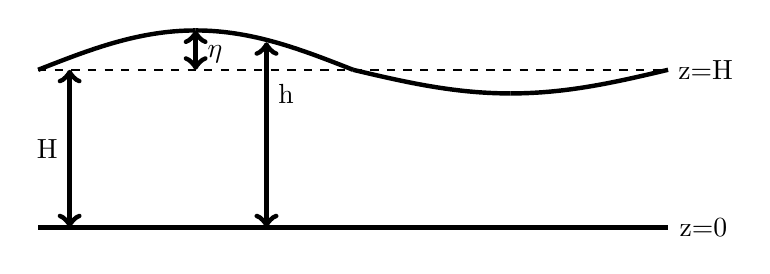
\begin{tikzpicture}
\draw[black,ultra thick] (-4,0) -- (4,0) node[anchor=west]{z=0};
\draw[black, dashed, thick] (-4,2) -- (4,2) node[anchor=west]{z=H};
\draw[black, ultra thick] (-4,2) sin (-2, 2.5);
\draw[black, ultra thick] (-2,2.5) cos (0, 2);
\draw[black, ultra thick] (0,2) sin (2, 1.7);
\draw[black, ultra thick] (2,1.7) cos (4, 2);
\draw[<-, black, line width=2pt] (-3.6,0) -- (-3.6,1) node[anchor=east] {H};
\draw[->, black, line width=2pt] (-3.6,1) -- (-3.6,2);
\draw[<-, black, line width=2pt] (-2,2) -- (-2,2.2) node[anchor=west] {$\eta$};
\draw[->, black, line width=2pt] (-2,2.2) -- (-2,2.5);
\draw[<-, black, line width=2pt] (-1.1,0) -- (-1.1,1.7) node[anchor=west] {h};
\draw[->, black, line width=2pt] (-1.1,1.7) -- (-1.1,2.35);
\end{tikzpicture}
\caption{Single layer shallow water system. H is the mean depth of the fluid, $\eta$ is the fluctuation from the mean, and $\mathrm{h} = \mathrm{H} + \eta$ is the total height of the fluid column.}
\label{fig:shallowwater}
\end{center}
\end{figure}
Shallow water theory uses hydrostatic balance for the vertical momentum equation. Since the density is assumed constant, the hydrostatic equation (\ref{eq:hydrostaticZ}) can be trivially integrated to express the pressure at a height $z$
\begin{align}
p(x,y,z,t) = -\rho g (z - \eta(x,y,t)).
\end{align}

The pressure gradient in the horizontal momentum equations is then simply
\begin{align}
\nabla_H p = \rho g \nabla_H \eta,
\end{align}
with $\nabla_H = (\partial/\partial x, \partial/\partial y)$. Thus the horizontal momentum equations in a single-layer shallow water system are 
\begin{align}
\frac{\partial \mathbf{u}}{\partial t} + (\mathbf{u} \cdot \nabla_H) \mathbf{u} + f \mathbf{k} \times \mathbf{u} = -g \nabla_H \eta.
\end{align}

Mass conservation can be derived by considering the mass flux into a cylindrical column of height $h$ and cross-sectional area $A$. Following Vallis \cite{Vallis2006},

\begin{align}
\text{Mass flux in} &= -\int_s \rho \mathbf{u} \cdot \text{d}S,
\end{align}
where $S$ is the area of the vertical boundary of the water column. If there is a net flux into the column, the height of the column must increase. Writing the surface area as $S = h\mathbf{n}\text{d}l$, where $\text{d}l$ is a line element of the closed curve $\mathcal{C}$ that encompasses the column and $\mathbf{n}$ is the outward pointing normal, then
\begin{align}
&= -\oint_{\mathcal{C}} \rho h\mathbf{u} \cdot \mathbf{n} ~\text{d}l,\\
&= -\int_A  \nabla \cdot (\rho\mathbf{u}h) ~\text{d}A.
\end{align}
The full mass conservation is then
\begin{align} 
&\frac{\text{d}}{\text{d}t} ~\int_V \rho \text{d}V = -\int_A  \nabla \cdot (\rho\mathbf{u}h) ~\text{d}A,\\
&\frac{\text{d}}{\text{d}t} ~\int_A \rho h \text{d}A = -\int_A  \nabla \cdot (\rho\mathbf{u}h)~ \text{d}A,\\
&\int_A \left[\rho \frac{\partial h}{\partial t} + \nabla \cdot (\rho\mathbf{u}h) \right]\text{d}A = 0.
\end{align}
Since the area integrated over is arbitrary, the integrand vanishes, leaving
\begin{align}
\frac{\partial h}{\partial t} + \nabla \cdot (\mathbf{u}h) = 0.
\end{align}

\subsection{Available Potential Energy}
\label{sec:APE}

In general, a conversion between kinetic, internal, and potential energy occurs in a flow. In the case of adiabatic, inviscid flow, the total energy is also conserved. In a stratified flow, not all of the potential energy can be converted to kinetic energy. Some of this potential energy is locked into the background state and is not free for extraction. The available potential energy, as the name suggests, is the amount of potential energy that is available for conversion. It is formally defined by Vallis as the difference between the potential energy of the initial state and the potential energy after an adiabatic arrangement to where the isentropic surfaces are flat.\\

\subsection{Helmholtz Decomposition}
\label{sec:helmholtz}
The domain-averaged kinetic energy can be written as 
\begin{align}
\text{E}_{k} = \frac{1}{2 V} \iiint \rho\left( \mathbf{u}\cdot \mathbf{u} + w^2\right) \text{d}V.
\end{align}
where $V$ is the volume of the domain. Since this is a cubic quantity in the unknowns, the energy is a sum over triads of wavevectors. To simplify this, since density perturbations from the base-state are small, we can instead consider only the base-state of the density, $\overline{\rho}$. The $w^2$ term can also be ignored because it is small compared to the horizontal velocities. The domain-averaged kinetic energy can now be written as
\begin{align}
\text{E}_{k} = \frac{1}{2V} \iiint \overline{\rho} \left(\mathbf{u}\cdot\mathbf{u}\right) \text{d}V. \label{eq:KE}
\end{align}

To study the kinetic energy contained at the different scales, it is useful to write the kinetic energy as a function of wavevectors. One way to do this, assuming horizontally periodic boundary conditions, is to use a two-dimensional discrete Fourier transform on the horizontal velocity fields at each vertical level, which yields a set of spectral coefficients. Through Parseval's theorem, the kinetic energy in the domain can be related to these spectra coefficients. That is, denoting $\widehat{q}(\mathbf{k})$ as the Fourier spectral coefficients of the field $q$, we have Parseval's theorem for a discrete Fourier transform

\begin{align}
 \frac{1}{N_x N_y} \sum_{m=0}^{N_x-1} \sum_{n=0}^{N_y-1} |q_{m,n}|^2 = \sum_{i=0}^{N_x-1}  \sum_{j=0}^{N_y-1} |\widehat{q}_{i,j}|^2.
\end{align}

With the kinetic energy is expressed as a function of the wavenumbers, a natural extension is to decompose the energy into its two dominant modes of motion: vortical and inertia gravity wave (IGW) motion. As outlined in Section \ref{sec:introduction}, one way to decompose the kinetic energy (equation \ref{eq:KE}) into slow vortical and fast wave motion is to apply a Helmholtz decomposition to the velocity fields. Helmholtz's theorem (for review, refer to \cite{Griffiths2013}) states that for a twice-differentiable bounded vector field $\mathbf{F}$ in $\mathbb{R}^2$, one can write the vector field as a combination of a rotational component $\mathbf{k} \times \nabla \mathbf{\psi}$, and an irrotational component $\Phi$,

\begin{align}
\mathbf{F} = \nabla \Phi + \mathbf{k}\times \nabla \mathbf{\psi}, \label{eq:helmholtz}
\end{align}

where $\psi$ is the streamfunction defined by $u = -\partial \psi/\partial y, v = \partial \psi/\partial x$. The resulting rotational field can be used as an analogue to the vortical motion, while the irrotational part can represent the inertia-gravity wave motion. To first compute the horizontal kinetic energy spectrum, which shows the kinetic energy as a function of the wavelength, we use a two-dimensional discrete Fourier transform. By Parseval's theorem, the kinetic energy in the domain can be related to the spectral coefficients given by the Fourier transform. Then using the Helmholtz decomposition, the kinetic energy spectrum can be written in terms of a rotational spectrum and a divergent spectrum.\\

 The divergent kinetic energy (DKE) for a specific horizontal wavevector is given by

\begin{align}
\text{E}_D(\mathbf{k}) = \frac{1}{2} \overline{\rho} \frac{ \bm{\widehat{\delta}}_{k,l} \cdot \bm{\widehat{\delta}}_{k,l}^*}{|\mathbf{k}|}, \label{eq:DKE}
\end{align}

where $\widehat{\delta}_{k,l} = ik\widehat{u}(\mathbf{k}) + il\widehat{v}(\mathbf{k})$ is the horizontal divergence, * denotes the complex conjugate, and $|\mathbf{k}| = \sqrt{k^2 + l^2}$ is the magnitude of the horizontal wavevector  $\mathbf{k} = (k,l)$. In similar fashion, the rotational kinetic energy (RKE) is written

\begin{align}
\text{E}_R (\mathbf{k})= \frac{1}{2} \overline{\rho} \frac{\bm{\widehat{\zeta}}_{k,l} \cdot \bm{\widehat{\zeta}}_{k,l}^*}{|\mathbf{k}|}, \label{eq:RKE}
\end{align}

with $\widehat{\zeta}_{k,l} = ik\widehat{v}(\mathbf{k}) - il\widehat{u}(\mathbf{k})$ as the vertical component of vorticity. When combined, equations (\ref{eq:DKE}) and (\ref{eq:RKE}) give

\begin{align}
\text{E}_R(\mathbf{k}) + \text{E}_D(\mathbf{k}) = \frac{1}{2} \overline{\rho} \left( |\widehat{u}(\mathbf{k})|^2 + |\widehat{v}(\mathbf{k})|^2 \right),
\end{align}

which is the total (rotational plus divergent) kinetic energy at a specific wavevector. 